\newif\ifvimbug
\vimbugfalse

\ifvimbug
\begin{document}
\fi

\exercise{Principal Component Analysis}
In this exercise, you will use the dataset \texttt{iris.txt}. It contains data from three kind of Iris flowers (`Setosa', `Versicolour' and `Virginica') with 4 attributes: sepal length, sepal width, petal length, and petal width. Each row contains a sample while the last attribute is the label ($0$ means that the sample comes from a `Setosa' plant, $1$ from a `Versicolour' and $2$ from `Virginica').
(You are allowed to use built-in functions for computing the mean, the covariance, eigenvalues and eigenvectors.)

\begin{questions}

%----------------------------------------------

\begin{question}{Data Normalization}{3}
Normalizing the data is a common practice in machine learning. Normalize the provided dataset such that it has zero mean and unit variance per dimension. Why is normalizing important?
Attach a snippet of your code. 

\begin{answer}
In machine learning some methods like PCA take the variance of the features as a criterion for dimensionality reduction. If the feature differ in their range, the means and the variances of the features will have a different scale. To achieve better comparability among the features it is common to normalize the data to unit variance and zero mean. The normalization can be achieved by applying the following formula to all datapoints $x_i$ for each feature separately:
\begin{equation*}
\frac{x_i-mean_{feature}}{standard\_deviation_{feature}}
\end{equation*}
We apply the normalization to the dataset according to the following code snippet.
\lstinputlisting[language=Python]{code/PCA_normalize.py}
\end{answer}

\end{question}

%----------------------------------------------

\begin{question}{Principal Component Analysis}{8}
Apply PCA on your normalized dataset and generate a plot showing the proportion (percentage) of the cumulative variance explained. 
How many components do you need in order to explain at least $95\%$ of the dataset variance? 
Attach a snippet of your code.
\begin{figure}[]
	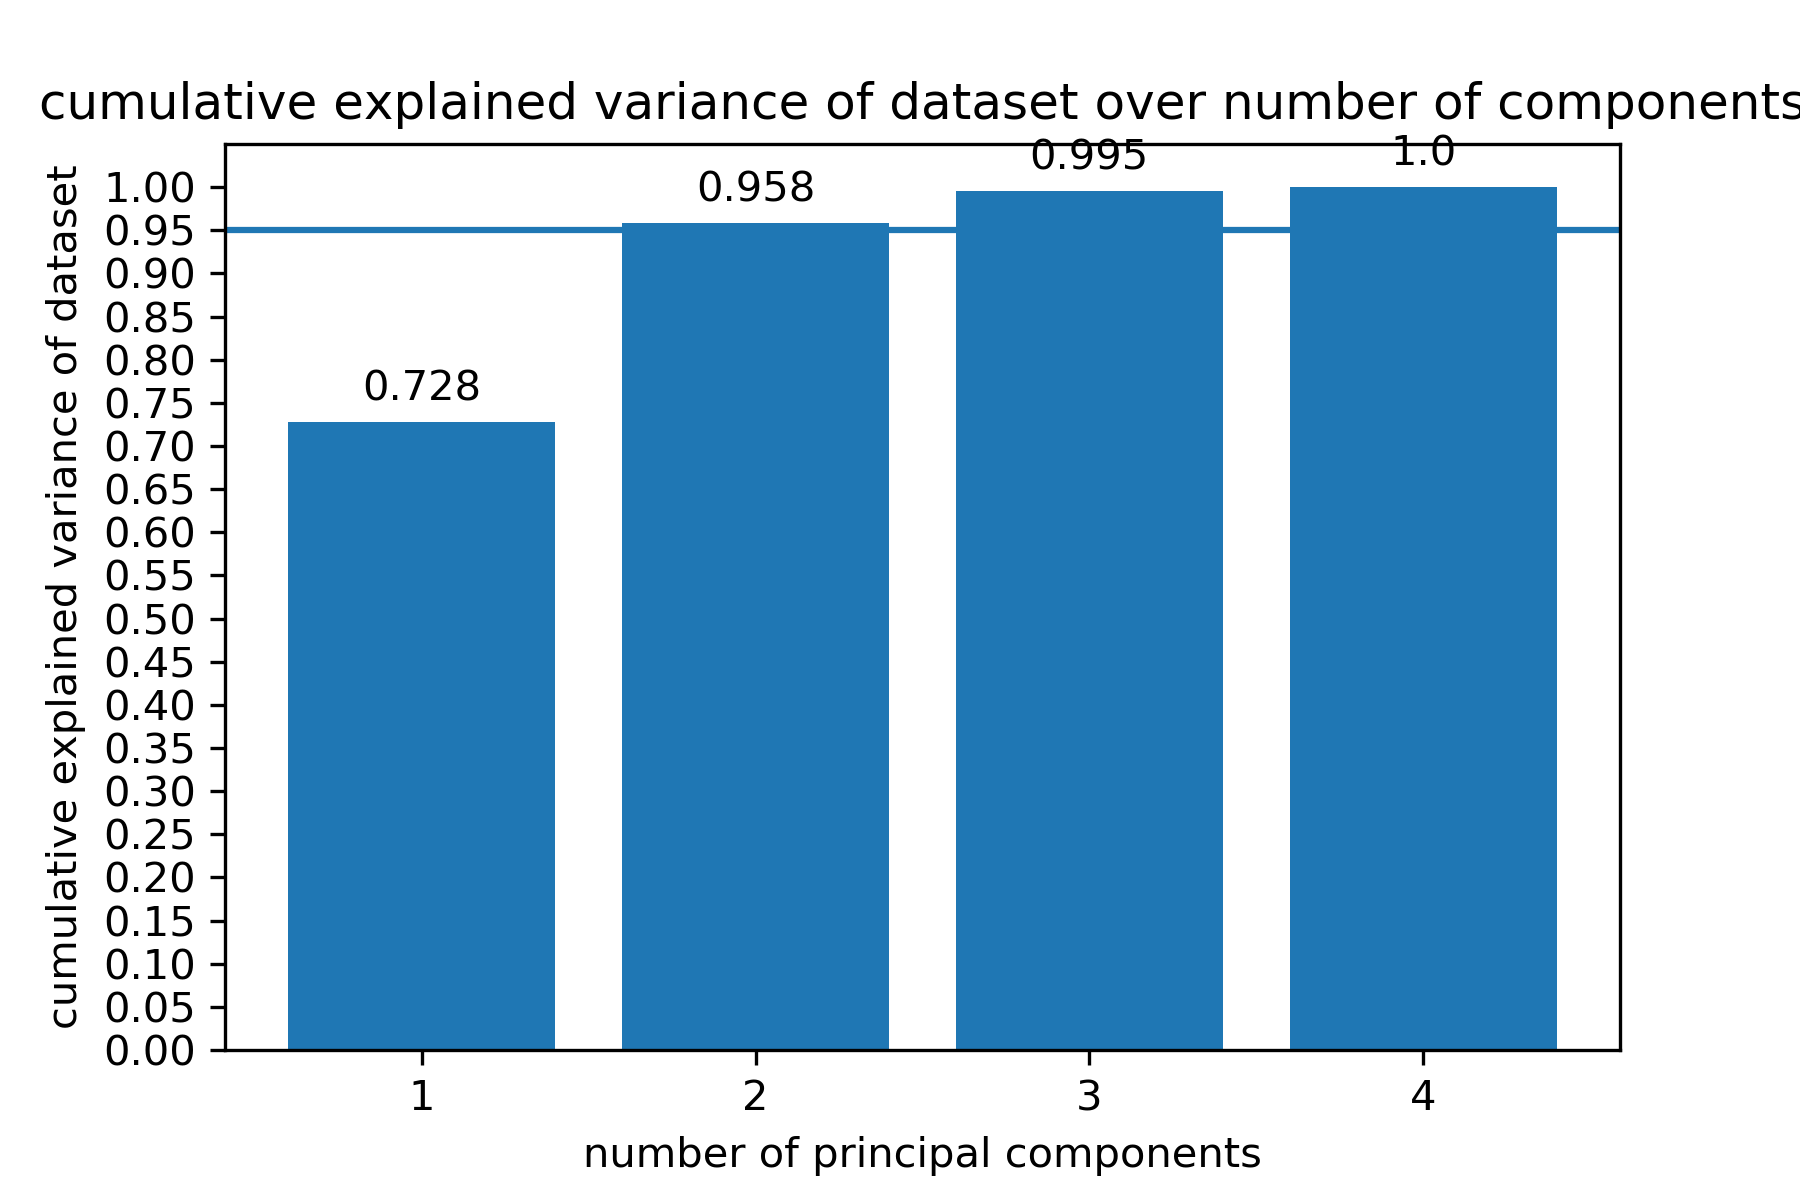
\includegraphics[width=0.8\linewidth]{pictures/explained_var_cumulative.png}
	\centering
	\caption{Cumulative explained variance of dataset over number of principal components.}
	\label{fig:1}
\end{figure}
\begin{answer}
As Figure \ref{fig:1} shows, by using two principal components we can explain 95,8\% of the cumulative variance. The following code snippet shows the code for doing the PCA and for plotting.
\lstinputlisting[language=Python]{code/PCA_explained_variance.py}
\end{answer}
\end{question}

%----------------------------------------------

\begin{question}{Low Dimensional Space}{6}
Using as many components as needed to explain $95\%$ of the dataset variance, generate a scatter plot of the lower-dimensional projection of the data. Use different colors or symbols for data points from different classes. 
What do you observe? Attach a snippet of your code.

\begin{answer}\end{answer}

\end{question}

%----------------------------------------------

\begin{question}{Projection to the Original Space}{6}
Reconstruct the original dataset by using different number of principal components. Using the normalized root mean square error (NRMSE) as a metric, fill the table below (error per input versus the amount of principal components used).

\begin{tabular}{c|r|r|r|r}
N. of components & $x_1$ & $x_2$ & $x_3$ & $x_4$ \\
\hline
1 & & & & \\
2 & & & & \\
3 & & & & \\
4 & & & &
\end{tabular}

Attach a snippet of your code.
(Remember that in the first step you normalized the data.)

\begin{answer}\end{answer}
\end{question}

\begin{question}[bonus]{Kernel PCA}{5}
Throughout this class we have seen that PCA is an easy and efficient way to reduce the dimensionality of some data. However, it is able to detect only linear dependences among data points. A more sophisticated extension to PCA, \emph{Kernel PCA}, is able to overcome this limitation. 
This question asks you to deepen this topic by conducting some research by yourself: explain what Kernel PCA is, how it works and what are its main limitations. Be as concise (but clear) as possible.

\begin{answer}\end{answer}
\end{question}

\end{questions}
